
\subsection{A Novel Sampling Structure}
After completing the BC-Shadow construction, the sampling space is significantly reduced. To count the bicliques, we can sample a subspace $\subspace$ and then sample an element $P$ from it to check $P$ forms a biclique. A simple approach might be to choose two vertex sets from $U$ and $V$ with sizes $p-|R_U|$ and $q-|R_V|$ respectively, but this naive method can still result in a large sampling space, \ie,$\binom{|S_U|}{p-|R_U|} \cdot \binom{|S_V|}{q-|R_V|}$. To further refine the process and make sampling more efficient, we need to impose additional constraints on $P$. In this section, we introduce a novel sampling structure, called zstar \cite{zigzag}, designed to efficiently sample elements from subspaces $(S_U,S_V,R_U,R_V) \in$ \shadow

For the convenience and improve the presentation of the general idea we introduce the concepts considering $G$ as the processing graph rather than the subspace $(S_U,S_V,R_U,R_V)$. Note that when applying for the proposed techniques to the subspace $(S_U,S_V,R_U,R_V)$ we need to consider the subgraph $G'(U',V',E')$ induced by $R_U,R_V$, $p$ as $p'$ where $p' = p-|R_U|$ and $q$ as $q'$ where $q' = q-|R_V|$.

For convenience, we assume without loss of generality that the vertices on each side of the bipartite graph $G'$ are arranged in some order.  Specifically, we have $u_1 \prec u_2 \prec \dots \prec u_{n_1}$ and $v_1 \prec v_2 \prec \dots \prec v_{n_2}$.We also assume that the $p \leq q$ because the same methods can be used when $p < q$. please note that for convenience, given examples in this paper does not consider the natural \red{is this correct?} ordering.

\begin{definition}
	\label{def:zstar}
	Given a bipartite graph $G(U, V, E)$ and integers $p,q,h$ , a $h$-zstar in $G$,is defined as an ordered vertex set
	\[
	Z = \{ u_{i_1}, v_{j_1}, u_{i_2}, v_{j_2}, \dots, u_{i_{h}}, v_{j_{h}}, \dots, v_{j_{h + (q - p)}} \}
	\]
	that satisfies the following conditions:
	\begin{enumerate}
		\item The number of vertices from the $U$ side is $h$, and the number of vertices from the $V$ side is $h + (q - p)$. \ie, $|Z|=2h+q-p$
		\item The vertices are ordered such that $i_1 < i_2 < \dots < i_{h}$ and $j_1 < j_2 < \dots < j_{h + (q - p)}$.
	\end{enumerate}
	Additionally, the length of a $(p, q)$-zstar is defined as $2h - 1$.
\end{definition}

 \begin{center}
	\begin{figure}
		
		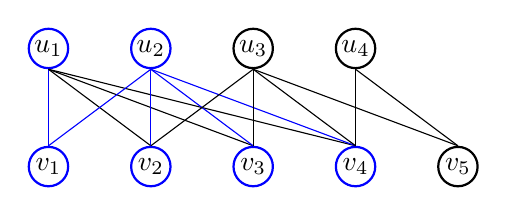
\begin{tikzpicture}[scale=1, every node/.style={circle, draw, minimum size=0.5cm, inner sep=0pt, line width=0.8pt}]
			
			% Nodes
			\node[draw=blue] (u1) at (0,1.5) {$u_1$};
			\node[draw=blue]  (u2) at (1.3,1.5) {$u_2$};
			\node (u3) at (2.6,1.5) {$u_3$};
			\node (u4) at (3.9,1.5) {$u_4$};
			
			\node [draw=blue] (v1) at (0,0) {$v_1$};
			\node [draw=blue] (v2) at (1.3,0) {$v_2$};
			\node [draw=blue] (v3) at (2.6,0) {$v_3$};
			\node [draw=blue] (v4) at (3.9,0) {$v_4$};
			\node (v5) at (5.2,0) {$v_5$};
			% Edges
			\draw [draw=blue] (u1.south) -- (v1.north);
			\draw (u1.south) -- (v2.north);
			\draw (u1.south) -- (v3.north);
			\draw (u1.south) -- (v4.north);
			\draw [draw=blue] (u2.south) -- (v1.north);
			\draw [draw=blue] (u2.south) -- (v2.north);
			\draw [draw=blue] (u2.south) -- (v3.north);
			\draw [draw=blue] (u2.south) -- (v4.north);
			
			\draw (u3.south) -- (v2.north);
			\draw (u3.south) -- (v3.north);
			
			\draw (u3.south) -- (v4.north);
			\draw (u3.south) -- (v5.north);
			
			
			\draw (u4.south) -- (v4.north);
			\draw (u4.south) -- (v5.north);
			
		\end{tikzpicture}
		\caption{An example for $Z_{(2,4)}$}
		\label{fig:z1} 
	\end{figure}
\end{center}


\begin{center}
	\begin{figure}
		
		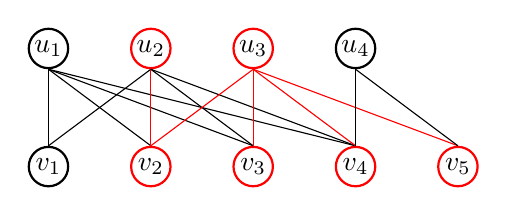
\begin{tikzpicture}[scale=1, 
			every node/.style={circle, draw, minimum size=0.5cm, inner sep=0pt, line width=0.8pt}
			]
			
			% Nodes
			\node (u1) at (0,1.5) {$u_1$};
			\node[draw=red] (u2) at (1.3,1.5) {$u_2$};
			\node [draw=red](u3) at (2.6,1.5) {$u_3$};
			\node (u4) at (3.9,1.5) {$u_4$};
			
			
			\node (v1) at (0,0) {$v_1$};
			\node[draw=red] (v2) at (1.3,0) {$v_2$};
			\node[draw=red] (v3) at (2.6,0) {$v_3$};
			\node [draw=red](v4) at (3.9,0) {$v_4$};
			\node [draw=red](v5) at (5.2,0) {$v_5$};
			
			% Edges
			\draw (u1.south) -- (v1.north);
			\draw (u1.south) -- (v2.north);
			\draw (u1.south) -- (v3.north);
			\draw (u1.south) -- (v4.north);
			\draw (u2.south) -- (v1.north);
			\draw[draw=red] (u2.south) -- (v2.north);
			\draw (u2.south) -- (v3.north);
			\draw (u2.south) -- (v4.north);
			
			\draw [draw=red](u3.south) -- (v2.north);
			\draw [draw=red](u3.south) -- (v3.north);
			
			\draw [draw=red](u3.south) -- (v4.north);
			\draw [draw=red](u3.south) -- (v5.north);
			
			
			\draw (u4.south) -- (v4.north);
			\draw (u4.south) -- (v5.north);
			
		\end{tikzpicture}
		\caption{Another for $Z_{(2,4)}$}
		\label{fig:z2} 
	\end{figure}
\end{center}

\red{edit examples}
Figures \ref{fig:z1} and \ref{fig:z2} shows two $2$-zstars in the example graph $G$.Note that the $2$-zstar in figure \ref{fig:z1} forms a (2,3)-bicique while figure \ref{fig:z2} does not form a (2,3)-biclique. In $2$-zstar shown in the figure \ref{fig:z1}, The primary purpose of designing zstar is to establish a correspondence between a biclique and a zstar such that every biclique has \textbf{exactly one} corresponding zstar. Note that every zstar may not have a corresponding biclique.

%\red{remove below}
%Let $\setbiclique(G) $ and $\Delta_{(p,q)}(G)$ denote  set of all \bicliques and  set of \zstars respectively in $G$ (we omit the subscript when the context is  clear), then the biclique density of $G$ is  calculated as
%
%\begin{equation}
%	\mathcal{\hat{B}}(G)  = \frac{cnt_{(p,q)}}{|\Delta|}
%\end{equation}

 let $\setzstar$ be the set of $h$-zstars in $G$.  We define a mapping $f: \setbiclique \to \Delta$ such that $f(b) = z$, where $B \in \setbiclique$ is a biclique and $Z \in \Delta$ is a \zstar. This mapping $f$ ensures that:

$$
\forall B \in \setbiclique, \exists Z \in \Delta \text{ such that } f(B) = Z,
$$

but

$$
\exists Z \in \Delta \text{ such that } \nexists B \in \setbiclique \text{ with } f(B) = Z.
$$

\begin{lemma}
	\label{lemma:zstar}
	given a $(p,q)$-biclique in $G$ with $p \leq q$, it contains exactly one \zstar if $p = h$
\end{lemma}

\begin{proof}
	The size of (p,q)-biclique is $p+q$ and by definition the size of \zstar is $2h+q-p$ .Hence a \biclique has exactly one \zstar.
\end{proof}

let $\mathcal{T}$ is the set of uniform \zstars sampled form $\Delta$ .


\begin{lemma}
	\label{lemma:zstarprob}
	let Z be a \zstar uniformly sampled from $\Delta$. The probability of $Z$ forms a  $(p,q)$-biclique in $G$ is $1/|\Delta|$
\end{lemma}

\begin{proof}
	As given in \ref{lemma:zstar} a \biclique contains exactly one \zstar,hence the lemma holds.
\end{proof}

Let $X(Z)$ be a binary random variable indicating whether a given \zstar Z forms a biclique, such that $X(Z) \in \{0,1\}$. For any Z, we define:

\[
X(Z) = \begin{cases}
	1 & \text{if } Z \text{ forms a biclique} \\
	0 & \text{otherwise}
\end{cases}
\]

Based on Lemma \ref{lemma:zstarprob}, we can construct an unbiased estimator for the count of bicliques by uniformly sampling Z from $\Delta$.


\begin{theorem}
 Consider $\mathcal{T}$, a set of $h$-zstars sampled uniformly from $\Delta$. The unbiased estimator for the count of $(p,q)$-bicliques in graph $G$, denoted as $\widehat{cnt}_{(p,q)}$, is given by:

	\[
	\estcnt = \frac{|\Delta| \sum_{Z \in \mathcal{T}} X(Z)}{|\mathcal{T}|}
	\]

	\begin{proof}[Proof]
		We proceed as follows:
		\begin{enumerate}
			\item By definition, we can establish that $\sum_{Z \in \mathcal{T}} X(Z) = \widehat{cnt}_{(p,q)}$
			\item This leads us to $\mathbb{E}[X(Z)] = \frac{\widehat{cnt}_{(p,q)}}{|\Delta|}$.
			\item Utilizing these results, we can demonstrate:
			\[
			\begin{aligned}
				\mathbb{E}\left[\estcnt\right] &= \mathbb{E}\left[\frac{|\Delta| \sum_{Z \in \mathcal{T}} X(Z)}{|\mathcal{T}|}\right] \\
				&= \frac{|\Delta|}{|\mathcal{T}|} \sum_{Z \in \mathcal{T}} \mathbb{E}[X(Z)] \\
				&= \cnt
			\end{aligned}
			\]
		\end{enumerate}
		Thus,  $\estcnt$ is an unbiased estimator for the count of $(p,q)$-bicliques.
	\end{proof}
\end{theorem}

\begin{algorithm}
	\label{algo:zstardp}
	\DontPrintSemicolon

	\caption{zstarDP$(G, p, q)$}
	\label{algo:zstardp}
	\KwIn{A bipartite graph $G(U, V, E)$ and integers $p$ and $q$}
	\KwOut{Dynamic programming table $dp$}
	\For{\textbf{each}  $e(v, u) \in E$}{
		Let $N_{>v}(u) \gets$ the set of neighbors of $u$ with vertex rank higher than the rank of $v$\;
		$dp[2][e(v, u)] \gets \binom{|N_{>v}(u)|}{q-p+1 }$\;
	}
	\For{$i = 3$ \textbf{to} $2h - 1$}{

		\For{\textbf{each}  $(v, u) \in E$}{
			\For{\textbf{each}  $(u', v)$ \textbf{where} $u' < u$}{
				$dp[i+1][(u',v)] \gets dp[i][(u',v)] + dp[i-1][e(v, u)]$\;
			}
		}

		\If{ $i \neq 2h-1$}{
			\For{\textbf{each}  $e(u', v) \in E$}{
				\For{\textbf{each}  $e(v', u')$ \textbf{where} $v' < v$}{
					$dp[i+1][e(v', u')] \gets dp[i+1][e(v', u')] + dp[i][e(u', v)]$\;
				}
			}

	}
		$i \gets i + 2$\;
	}

	\Return{$dp$};
\end{algorithm}


\textbf{Counting and Sampling zstars:} Reminding that we assume that $p \leq q$ and $h = p$, To maximize the utility of zstars, it is essential to efficiently count the number of \zstars in a graph $G$. We propose an efficient dynamic programming approach for counting \zstars, inspired by \cite{zigzag} . As defined in \ref{def:zstar}, If every zstar originates from a node $u$ , then the total count of zstars can be determined by summing the zstars that start from each $u$ in the set $U$.Let $dp[i][(u,v)]$ represent the number of zstars with length $i$ starting from $(u, v)$, where $i \in [2,2h-1] $. Then the number of zstars with length $2h-1$ starting from $u$ can be represented as $\sum_{v \in N(u)} dp[2h - 1][e(u, v)]$. Then the total zstars in $G$ is $\sum_{e \in E} dp[2h - 1][e(u, v)]$.

We noticed that $dp[i][e(u, v)]$ can also be computed using a dynamic programming algorithm. The core concept of our DP approach is that each zstar with the length of $i$ beginning from $u$ is built upon the zstar of length $i - 1$ starting from node $v$ when i > 2.Therefore, we have below recursion equation:

\begin{equation}
	\label{dpcount}
	\begin{cases}
		dp[i][e(u, v)] \gets \sum_{u' \in N_{> u}(v)} dp[i - 1][e(v, u')], \\
		dp[i - 1][e(v, u')] \gets \sum_{v' \in N_{> v}(u')} dp[i - 2][e(u', v')], \\
		dp[2][e(v, u)] \gets \binom{|N_{>u}(v)|}{q - p} \\
	\end{cases}
\end{equation}


Note that notations  $dp[i][e(u, v)] $ and $dp[i][e(v, u)] $ in equation (\ref{dpcount}) are different to each other. Algorithm \ref{algo:zstardp} outlines the steps for counting $h$-zstars. The algorithm takes as input the graph $G$ and two integers, $p$ and $q$, and produces a dynamic programming table that records the zstar counts for each edge in $G$, with zstar lengths ranging from 2 to $2h-1$.


The initial time complexity of Algorithm \ref{algo:zstardp} is $ O(h\cdot d_{max} \cdot |E|) $, where $ d_{max} $ is the maximum degree of the input graph $G$ and $ h = \min(p, q) $. This is inefficient for large graphs since $ d_{max} $ could be equal to number of vertices in either side, making the algorithm impractical for large graphs. To address this, we apply a differential-interval updating technique that reduces the time complexity to $ O(h \cdot |E|) $.

Consider the dynamic programming table at level $ i $, denoted as $ dp[i] $, represented as a sequence $ \{a_1, a_2, \dots, a_n\} $, where $ a_j = dp[i][e_j] $ corresponds to an edge $ e_j $. We transform this into a difference sequence $ \{b_1, b_2, \dots, b_n\} $, where $ b_1 = a_1 $ and $ b_j = a_j - a_{j-1} $ for $ j = 2 $ to $ n $. Each $ a_j $ is reconstructed by computing the prefix sum: $ a_j = \sum_{k=1}^{j} b_k $.

In the algorithm, updates occur when $ i $ is odd (for edges $ e(v, u') $ where $ u' > u $) and when $ i $ is even (for edges $ e(u, v') $ where $ v' > v $). These updates increment $ a_j $ over specific intervals. By using the difference sequence $ \{b_1, b_2, \dots, b_n\} $, we can efficiently apply these interval updates by modifying $ b_l \mathrel{+}= w $ and $ b_{r+1} \mathrel{-}= w $ for the range $[l, r]$, where $w$ is the value we need to add. After applying all updates, the original $ dp[i] $ is reconstructed by computing prefix sums.

This technique reduces the per-update time from $ O(k) $, where $ k $ is the number of edges in the interval, to $ O(1) $, leading to a total time complexity of $ O(h \cdot |E|) $.

\textbf{sampling a zstar}: Since we have efficient method to count the zstars in $G$ ,now we need to efficiently sample a zstar uniformly at random from $\setzstar$, ensuring that each zstar has an equal probability $\frac{1}{|\setzstar|}$ of being selected. To achieve this, we utilize the DP table $dp[i][e(u,v)]$, which records the number of partial zstars of length $i$ ending at edge $e(u,v)$.


We present an efficient method to uniformly sample a $h$-zstar from the bipartite graph $G$, leveraging the dynamic programming counts obtained earlier. The central challenge in uniformly generating a $h$-zstar is to establish the correct probability distribution over all possible zstars in $G$. By utilizing the counts computed in the dynamic programming table, we can construct this probability distribution effectively.

Recall that the total number of $h$-zstars in $G$ is given by:

\begin{equation} |\setzstar| = \sum_{e(u,v) \in E} dp[2h - 1][e(u,v)], \end{equation}

where $dp[2h - 1][e(u,v)]$ denotes the number of zstars of length $2h - 1$ starting from edge $e(u,v)$. This total count allows us to define the probability of an edge $e(u,v)$ being the starting edge of a zstar $Z$ as:

\begin{equation} P(e(u,v)) = \frac{dp[2h - 1][e(u,v)]}{\sum_{e(u,v) \in E} dp[2h - 1][e(u,v)]} \end{equation}

Once the starting edge is selected, the subsequent edges in the zstar can be determined recursively. Specifically, for the next edge $e(v,u')$ where $u' \in N_{>u}(v)$ (the neighbors of $v$ with a higher rank than $u$), the conditional probability of choosing $e(v,u')$ given that $e(u,v)$ is the current edge is:

\begin{equation} P(e(v,u') \mid e(u,v)) = \frac{dp[2h - 2][e(v,u')]}{dp[2h - 1][e(u,v)]}. \end{equation}

\noindent This recursive method continues for each subsequent edge in the zstar, decrementing $ i $ from $ 2h - 1 $ down to $ 2 $. By this stage, we have sampled $ p $ vertices from the $ U $ side and $ p - 1 $ vertices from the $ V $ side. To complete the h-zstar, we need to select the remaining $ q - p + 1 $ vertices from $ V $.

Given the last edge $ e(u, v) $ selected in the recursive procedure, we proceed by choosing $ q - p + 1 $ additional vertices from the set $N_{>v}(u)$. To maintain uniformity, each vertex $ v' $ in $ N_{>v}(u) $ is selected with equal probability:

\begin{equation}
	P(v') = \frac{1}{\left| N_{>v}(u) \right|}.
\end{equation}

By uniformly sampling these vertices, we ensure that all possible combinations are equally likely, thus preserving the uniformity of the overall sampling process. We summarise these steps in algorithm \ref{algo:samplingzstar}.




%
%\begin{algorithm}
%	\DontPrintSemicolon
%	\label{algo:samplingzstar}
%	\caption{Sampling a ZStar}
%	\KwIn{A bipartite graph $G=(U,V,E)$, integesr $h,q$}
%	\KwOut{}
%	Set the distribution $\mathcal{D}$ over edges where $p(e(u,v)) = \frac{dp[2h-1][e(u,v)]}{\sum e(u,v) dp[2h-1][e(u,v)]};$ \\
%	Sample an edge $e(u,v)$ according to $\mathcal{D}$;\\
%	$Z \gets \{e(u,v)\};$ \\
%	\For{$i = 2h-2$ \textbf{to} $2$}{
%		$E' \gets \{e(v,u') | u' \in N(v) \wedge u' > u\};$ \\
%		Set the distribution $\mathcal{D}$ over $E'$ where $p(e) = \frac{dp[i][e]}{\sum_{e \in E'} dp[i][e]};$ \\
%		Sample an edge $e(v,u')$ according to $D$; \\
%		$Z \gets Z \cup \{e(v,u')\};$ \\
%
%
%		$E' \gets \{e(u',v') | v' \in N(u') \wedge v' > v \};$ \\
%		Set the distribution $D$ over $E'$ where $p(e) = \frac{dp[i-1][e]}{\sum_{e \in E'} dp[i-1][e]};$ \\
%		Sample an edge $e(u',v')$ according to $\mathcal{D}$; \\
%		$Z \gets Z \cup \{e(u',v')\};$ \\
%		$u \gets u';$ $v \gets v';$\\
%		$i \gets i-2;$\\
%	}
%		$E' \gets \{e(u',v'') | v'' \in N(u') \wedge v'' > v' \};$ \\
%	\For{$j = q-h$ \textbf{to} $1$}{
%		Set the distribution $\mathcal{D}$ over $E'$ where $p(e) = \frac{1}{|E'|};$ \\
%		Sample an edge $e(u',v'')$ according to $\mathcal{D}$ \\
%		$E' \gets E'  \;  \backslash  \; e(u',v'')$
%	}
%	\Return{$Z;$}
%\end{algorithm}

\begin{algorithm}[]
	\DontPrintSemicolon
	\caption{Sampling a Z-Star}
	\label{algo:samplingzstar}
	\KwIn{A bipartite graph $G=(U,V,E)$, integers $p$, $q$}
	\KwOut{A uniformly sampled zstar $Z$}
	Set the distribution $\mathcal{D}$ over edges where $p(e(u,v)) = \frac{dp[2h-1][e(u,v)]}{\sum_{e(u,v) \in G} dp[2h-1][e(u,v)]};$ \\

	Sample an edge $e(u_0, v_0)$ according to $\mathcal{D}$\;
	Initialize $Z \gets \{ u_0, v_0 \}$, $k \gets 0$ \;

	\tcp{Recursive construction of zstar}
	\For{$i = 2h - 2$ \textbf{down to} $2$ \textbf{step} $-1$}{
		\eIf{$i$ is even}{
			\tcp{Sampling edge from $V$ to $U$}
			$E' \gets \{ e(v_k, u') \mid u' \in N_{>u_k}(v_k) \}$\;
			Set the distribution $\mathcal{D}$ over $E'$ where:
			\[
			P(e(v_k, u')) = \dfrac{dp[i][e(v_k, u')]}{dp[i+1][e(u_k, v_k)]}
			\]
			Sample an edge $e(v_k, u_{k+1})$ according to $\mathcal{D}$\;
			Append $u_{k+1}$ to $Z$\;

		}{
			\tcp{Sampling edge from $U$ to $V$}
			$E' \gets \{ e(u_{k+1}, v') \mid v' \in N_{>v_k}(u_{k+1}) \}$\;
			Set the distribution $\mathcal{D}$ over $E'$ where:
			\[
			P(e(u_{k+1}, v')) = \dfrac{dp[i][e(u_{k+1}, v')]}{dp[i+1][e(v_k, u_{k})]}
			\]
			Sample an edge $e(u_{k+1}, v_{k+1})$ according to $\mathcal{D}$\;
			Append $v_{k+1}$ to $Z$\;
			$k \gets k + 1$\;
		}

	}

	\tcp{Add remaining vertices from $V$}
	$V_{\text{rem}} \gets \{ v' \in N_{>v_k}(u_{k+1}) \}$\;
	Uniformly select $q - p + 1$ vertices from $V_{\text{rem}}$ without replacement; \\
	Append the selected vertices to $Z$\;
	\Return{$Z$}
\end{algorithm}



